%%%%%%%%%%%%%%%%%%%%%%%%%%%%%%%%%%%%%%%%%%%%%%%%%%%%%%%%%%%%%%%%%%%%%%%%%
% latex ewald
% xdvi ewald &
% dvips -D600 ewald.dvi -o ewald.ps
%%%%%%%%%%%%%%%%%%%%%%%%%%%%%%%%%%%%%%%%%%%%%%%%%%%%%%%%%%%%%%%%%%%%%%%%%
\documentclass[11pt]{article}
\usepackage{graphicx}
\usepackage{fullpage}
\usepackage{amsmath}
\usepackage{amssymb}
\usepackage{times}
\newcommand{\ProtoMol}{\textsc{ProtoMol }}
\newcommand{\erf}{\mbox{erf}}
\newcommand{\erfc}{\mbox{erfc}}
\providecommand{\bm}[1]{\mbox{\boldmath${#1}$}}
\providecommand{\textinmath}[1]{\mbox{#1}}
\providecommand{\textinmathss}[1]{\mbox{\scriptsize #1}}
\author{Thierry Matthey\\{\tt matthey@ii.uib.no}}

\title{Plain Ewald and PME}
%%%%%%%%%%%%%%%%%%%%%%%%%%%%%%%%%%%%%%%%%%%%%%%%%%%%%%%%%%%%%%%%%%%%%%%%%
\begin{document}
%%%%%%%%%%%%%%%%%%%%%%%%%%%%%%%%%%%%%%%%%%%%%%%%%%%%%%%%%%%%%%%%%%%%%%%%%
\maketitle
%%%%%%%%%%%%%%%%%%%%%%%%%%%%%%%%%%%%%%%%%%%%%%%%%%%%%%%%%%%%%%%%%%%%%%%%%

%%%%%%%%%%%%%%%%%%%%%%%%%%%%%%%%%%%%%%%%%%%%%%%%%%%%%%%%%%%%%%%%%%%%%%%%%
\section{Introduction}
%%%%%%%%%%%%%%%%%%%%%%%%%%%%%%%%%%%%%%%%%%%%%%%%%%%%%%%%%%%%%%%%%%%%%%%%%
\subsection{Standard Ewald summation\label{sec:ewald}}

A general potential energy function $U$ of a system of $N$ particles with an 
interaction potential  $\phi (\vec{x}_{ij}+\vec{n})$ and periodic boundary
conditions can be expressed as 
\begin{equation}
 U = \frac{1}{2}\sideset{}{^\dag}\sum_{\vec{n}} \sum_{i=1}^{N} \sum_{j=1}^{N} 
\phi (\vec{x}_{ij}+\vec{n}), 
\label{eq:potentialpbc}
\end{equation}
where $\sum_{\vec{n}}$ is the sum over all lattice vectors 
$\vec{n} = (L_{x}n_{x},L_{y}n_{y},L_{z}n_{z})$, $n_{x,y,z} \in \mathbb{N}$ and
$L_{x,y,z}$ are the dimensions of the unit MD cell and
$\vec{x}_{ij}=\vec{x}_{j}-\vec{x}_{i}$. The ``daggered''
($^\dag$) summation indicates the exclusion of all pairs $i=j$ inside the
original unit MD cell ($\vec{n} = \vec{0}$). Most molecular force fields
provide exclusion schemes to exclude additional pairs, e.g., the
so-called {\it 1-3 exclusion} excludes directly connected pairs and
pairs with a direct common neighbor. Furthermore, some exclusion schemes
may also modify the potential by a factor for certain pairs.

If the potential $\phi$ satisfies 
\begin{equation}
| \phi(\vec{x}) | \leq A|\vec{x}|^{-3 - \epsilon}
\label{eq:absconvergent}
\end{equation}
for large enough $\vec{x}$ and  $A > 0$ and $\epsilon > 0$, then
the sum in Eq.\ (\ref{eq:potentialpbc}) is absolute
convergent\footnote{The sum converges and does not depend on the order of
summation.}.

Inequality (\ref{eq:absconvergent}) is not satisfied by the Coulomb
potential $\phi(\vec{x}_{ij}) = cq_iq_j |\vec{x}_{ij}|^{-1}$, such that the
infinite lattice sum in Eq.\ (\ref{eq:potentialpbc}) is only conditionally
convergent\footnote{The convergence of the sum depends on the order of
summation.}. In case of the Lennard-Jones potential, the
sum is absolutely convergent.

The well-known Ewald summation method~\cite{Ewal21} is in
general useful in systems with large, spatial potential differences,
where the summation over one unit cell does not converge sufficiently,
i.e., the lattice sum is not absolutely convergent. The lattice sum
with the Coulomb potential is usually expressed as
\begin{equation}
\label{eq:coulombpbc}
U^{\textinmathss{electrostatic}} =\frac{1}{4 \pi \epsilon_0} \frac{1}{2}\sideset{}{^\dag}\sum_{\vec{n}}
\sum_{i=1}^{N}\sum_{j=1}^{N} \frac{q_{i}q_{j}}{| \vec{x}_{ij} +  \vec{n} |}.
\end{equation}
To overcome the conditionally and insufficient convergence of
Eq.\ (\ref{eq:coulombpbc}), the sum is split into two parts by the following trivial
identity 
\begin{equation}
\label{eq:identity}
\frac{1}{r} = \frac{f(r)}{r} + \frac{1-f(r)}{r}.
\end{equation}
The basic idea is to separate the fast variation part for small $r$ and
the smooth part for large $r$. In particular, the first part should decay
fast and be negligible beyond some cutoff distance, whereas the second part should
be smooth for all $r$, such that its Fourier transform can be
represented by a few terms. Ewald~\cite{Ewal21} suggested to
choose a Gaussian convergence factor $g(s,\vec{n}) = e^{-s|\vec{n}|^2}$
such that the sum becomes (see~\cite{LPSm80} for a detailed mathematical
derivation of the Ewald summation)
%
\begin{eqnarray}
\label{eq:ewald}
U^{\textinmathss{electrostatic}} & = & \underbrace{\frac{1}{4 \pi \epsilon_0} \frac{1}{2}\sideset{}{^\dag}\sum_{\vec{n}}
\sum_{i=1}^{N}\sum_{j=1}^{N}  q_{i}q_{j} \frac{\erfc (\alpha | \vec{x}_{ij}
+  \vec{n} |)}{| \vec{x}_{ij} +  \vec{n} |}}_{\textinmath{Real-space
term}}\nonumber\\
& + & \underbrace{\frac{1}{\epsilon_0 V}\frac{1}{2}\sum_{\vec{k} \neq
0}\frac{1}{\vec{k}^2}e^{-\frac{\vec{k}^2}{4 \alpha^2}}\left [ \left |
\sum_{i=1}^{N} q_i \cos (\vec{k} \cdot \vec{x}_i) \right |^2 + \left |
\sum_{i=1}^{N} q_i \sin (\vec{k} \cdot \vec{x}_i) \right |^2 \right
]}_{\textinmath{Reciprocal-space term}}\nonumber\\
& - & \underbrace{\frac{1}{4 \pi \epsilon_0} \frac{1}{2} \sideset{}{^{\dag ^{-1}}}\sum_{j=1}^{M}
\sum_{k=1}^{N_j} \sum_{l=1}^{N_j}  q_{j_k} q_{j_l}
\frac{\erf( \alpha | \vec{x}_{j_k j_l} |)}{|
\vec{x}_{j_k j_l}| }}_{\textinmath{Intra-molecular self energy}}\\
&~-~& \underbrace{\frac{\alpha}{4 \pi^\frac{3}{2}
\epsilon_0}\sum_{i=1}^{N} q_i^2}_{\textinmath{Point
self energy}} ~-~  \underbrace{\frac{1}{8 \epsilon_0 V \alpha ^2} \left |
\sum_{i=1}^N q_i \right |^2}_{\textinmath{Charged system term}} +
\; \underbrace{\left [  \frac{1}{6 \epsilon_0 V} 
                    \left | \sum_{i=1}^N q_i \bm{x}_i 
                    \right |^2 \right ]}_{\textinmath{Surface dipole term}}.\nonumber
\end{eqnarray}
Here, $\alpha$ is the splitting parameter of the real and reciprocal
part. For an optimal $\alpha$ the Ewald summation scales as
$\mathcal{O}(N^{\frac{3}{2}})$~\cite{Ewal21,Finc94,PePL88}
in Eq.\ (\ref{eq:ewald-alpha}). $^{\dag^{-1}}$ is the ``inverse
daggered'' summation. The intra-molecular self term corrects 
interactions on the same molecule, which are implicitly included in
the reciprocal-space term, but are not required in the exclusion
model. Self interactions are canceled out by the self point
term. The charged system term is only necessary if the total net
charge of the system is non-zero. Note, that some MD systems have an
additional surface dipole term to model dipolar systems more
accurately~\cite{LPSm80,WaHo01}. This term is not
suited for mobile ions, since it will create discontinuities in the
energy and force contributions when ions cross boundaries. The meaning of the symbols is
\begin{tabbing}
\rule{2cm}{0cm} \= \rule{2cm}{0cm} \=\\
\> $\bm{n}$        \> lattice vector of periodic cell images \\
\> $\bm{k}$        \> reciprocal lattice vector of periodic cell images \\
\> $k$             \> modulus of $\bm{k}$ \\
\> $i,j$           \> absolute indices of all charged sites \\
\> $n$             \> index of molecules \\
\> $\kappa,\lambda$ \> indices of sites within a single molecule \\
\> $N$             \> total number of charged sites \\
\> $M$             \> total number of molecules \\
\> $N_j$           \> number of sites on molecule $j$ \\
\> $q_i, q_j$           \> charge on absolute site $i$, $j$ \\
\> $q_{m\kappa}$   \> charge on site $\kappa$ of molecule $m$ \\
\> $\bm{x}_i$      \> Cartesian co-ordinate of site $i$ \\
\> $\bm{x}_{ij}$   \> $\bm{x}_j - \bm{x}_i$ \\
\> $\alpha$        \> real/reciprocal space partition parameter
\end{tabbing}


The electrostatic force on particle $i$ is given by
%
\begin{eqnarray}
\label{eq:ewald-force}
F^{\textinmathss{electrostatic}}_i &=& - \nabla_{\vec{x}_i} U^{\textinmathss{electrostatic}} \nonumber\\
& = & \underbrace{\frac{q_i}{4 \pi \epsilon_0} \sideset{}{^\dag}\sum_{\vec{n}}
\sum_{j=1}^{N} q_j \left [ \frac{\erfc( \alpha |
\vec{x}_{ij} + \vec{n} |)}{|\vec{x}_{ij} +\vec{n} | } + \frac{2
\alpha}{\sqrt{\pi}}e^{- \alpha^2 | \vec{x}_{ij} + \vec{n} |^2} \right ]
\frac{\vec{x}_{ij} + \vec{n}}{| \vec{x}_{ij} + \vec{n}
|^2}}_{\textinmath{Real-space term}} \nonumber \\
& &\hspace{-3cm}+~  \underbrace{\frac{1}{\epsilon_0 V} \sum_{\vec{k} \neq 0} q_i
\frac{\vec{k}}{\vec{k}^2} e^{-\frac{\vec{k}^2}{4 \alpha^2}} \left [  \sin(k
\cdot r_i) \sum_{j=1}^{N} q_j \cos(\vec{k} \cdot \vec{x}_j) - \cos(k
\cdot r_i) \sum_{j=1}^{N} q_j \sin(\vec{k} \cdot \vec{x}_j) \right
]}_{\textinmath{Reciprocal-space term}}\nonumber\\
& + & \underbrace{\frac{q_i}{4 \pi \epsilon_0} \frac{1}{2} \sideset{}{^{\dag ^{-1}}}\sum_{j}
    q_j \left [ \frac{2 \alpha}{\sqrt{\pi}}e^{-
\alpha^2 | \vec{x}_{ij}  |^2} -\frac{  \erf( \alpha | \vec{x}_{ij}
|)}{|\vec{x}_{ij}|} \right ] \frac{\vec{x}_{ij}}{| \vec{x}_{ij}
|^2}}_{\textinmath{Intra-molecular term}}\\
  & + & \underbrace{\left [ \frac{q_i}{6 \epsilon_0 V} \left (
        \sum_{j=1}^N q_j \bm{x}_j \right ) \right
    ]}_{\textinmath{Surface dipole term}} 
\end{eqnarray}
%
Furthermore, the Ewald method can also be used for van der Waals
interactions~\cite{ChCG97,KaGo89} and several other
potentials~\cite[pp.~237-256]{Gao98},\cite{LPSm80}.
The computational efficiency and
accuracy for 2-dimensional periodic boundary conditions in a
3-dimensional system is discussed in~\cite{KaMi01}. The case with 1-dimensional periodic
boundary conditions is addressed in~\cite{LaHC01}.
To some extent, vacuum systems can be treated by imposing periodic
boundary conditions. The dimensions
of the original unit cell are chosen big enough, such that the
contributions between cell images are negligible. In practice, the
dimensions of the unit cell are a factor of $100$ larger than the minimal
bounding box of particles.\\

The real, reciprocal and correction terms (the
last 3 terms of Eq.\ (\ref{eq:ewald}))  can be
evaluated independently. This is typically used in combination with MTS to
split the force into fast and slow varying parts.
Furthermore, the real space term supports
not only simple truncation, but also switching functions to modify the
potential. The implementation supports parallelism (range computation)
for the real, reciprocal and correction terms. It handles MD systems for both vacuum and periodic boundary
conditions. Due to the relatively expensive sine and cosine functions,
\ProtoMol\ uses look-up tables and the addition theorem to evaluate
$\cos(\vec{k} \cdot \vec{x}_i)$ and $\sin(\vec{k} \cdot \vec{x}_i)$ 
more efficiently in Eqs.\ (\ref{eq:ewald}) and (\ref{eq:ewald-force});
$\erf(x)$ and $\erfc(x)$ are by default not approximated, since the
system platforms provide a well optimized implementation.

%%%%%%%%%%%%%%%%%%%%%%%%%%%%%%%%%%%%%%%%%%%%%%%%%%%%%%%%%%%%%%%%%%%%%%%%
\subsubsection*{Uniform Sheet Correction}
%%%%%%%%%%%%%%%%%%%%%%%%%%%%%%%%%%%%%%%%%%%%%%%%%%%%%%%%%%%%%%%%%%%%%%%%

The 5th term in Equation~\ref{eq:ewald} is necessary only if the system
has a non-zero net electric charge, and is useful in special cases such
as framework systems.  

In a periodic system the electrostatic energy is finite only if the
total electric charge of the MD cell is zero.  The reciprocal space
sum in Equation~\ref{eq:ewald} for $\bm{k}=0$ takes the form
\[\frac{1}{k^2}e^{-\frac{k^2}{4 \alpha^2}} \left | \sum_{i=1}^{N} q_i
 \right |^2\] which is zero in the case of electroneutrality but
infinite otherwise.  Its omission from the sum in
Equation~\ref{eq:ewald} is physically equivalent to adding a uniform
jelly of charge which exactly neutralizes the unbalanced point
charges.  Though the form of the reciprocal space sum is
unaffected by the uniform charge jelly the real-space sum is not.  The
real-space part of the interaction of the jelly with each point charge
as well as the self-energy of the jelly itself must be included giving
the fifth term in Equation~\ref{eq:ewald}.

%%%%%%%%%%%%%%%%%%%%%%%%%%%%%%%%%%%%%%%%%%%%%%%%%%%%%%%%%%%%%%%%%%%%%%%%
\subsubsection*{Surface Dipole Term}
%%%%%%%%%%%%%%%%%%%%%%%%%%%%%%%%%%%%%%%%%%%%%%%%%%%%%%%%%%%%%%%%%%%%%%%%

The optional final term in Equations~\ref{eq:ewald} 
and~\ref{eq:ewald-force} if used performs the calculations under
different periodic boundary conditions.  It was suggested by De Leeuw,
Perram and Smith\cite{} in order to accurately model
dipolar systems and is necessary in any calculation of a dielectric
constant. 

The distinction arises from considerations of how the imaginary set of
infinite replicas is constructed from a single copy of the MD 
box\cite[pp 156-159]{}.  Consider a near-spherical cluster
of MD cells.  The ``infinite'' result for any property is the limit of
its ``cluster'' value as the size of the cluster tends to infinity.
However this value is non-unique and depends on the dielectric
constant, $\epsilon_s$ of the physical medium surrounding the cluster.
If this medium is conductive ($\epsilon_s=\infty$) the dipole
moment of the cluster is neutralized by image charges, whereas in a
vacuum ($\epsilon_s=1$) it remains.  It is trivial to show that
in that case the dipole moment per unit volume (or per MD cell) does
\emph{not} decrease with the size of the cluster.

The final term in Equation~\ref{eq:ewald} is just the dipole energy,
and ought to be used in any calculation of the dielectric constant of
a dipolar molecular system.   Note that as it represents the
dipole at the surface of the cluster the system is no longer truly
periodic.

Conversely it \emph{must not} be used if the simulated system contains
mobile ions.  Consider an ion crossing a periodic boundary and jumping
from one side of the MD cell to another.  In that case the dipole
moment of the MD cell changes discontinuously.   Because of the
surface dipole term the calculation would model a discontinuous
macroscopic change in the dipole moment of the whole system caused by
an infinite number of ions jumping an infinite distance.  This is
manifested in practice by a large and discontinuous change in the
energy of the system and on the force on each charge within it.

This situation is completely non-physical but is easily avoided.
However the problem may also arise more subtly even when there are no
mobile ions if a framework is being simulated.  The framework is treated as a set of
discrete, but fixed atoms rather than a molecular unit.  If the shape
of the unit cell is allowed to vary then ions constituting the
framework may indeed cross MD cell boundaries causing the
aforementioned problems.



Figure~\ref{fig:relativemaxerror} shows the maximum relative force
error of the Ewald method for different accuracy parameters $\epsilon$
compared to the Ewald method with accuracy parameter $\epsilon =
10^{-18}$ (see Eqs.\ (\ref{eq:ewald-alpha}-\ref{eq:ewald-kc})) under
periodic boundary conditions. There was no significant improvement for
smaller $\epsilon$, which is obvious, due to machine precision of
order $10^{-16}$. The maximum relative error of the Ewald
implementation compared against the direct method in vacuum is less
than $10^{-15}$ with an accuracy parameter $\epsilon = 10^{-18}$ and a
unit MD cell $10^8$ times larger than the minimal bounding box of
particles. Figure~\ref{fig:timmeaccuracy} illustrates the
corresponding normalized run-time. Figure~\ref{fig:energydriftPBC}
shows  excellent energy conservation with a maximum relative force
error of order $10^{-10}$. Moldy~\cite{Refs00} was also used for
further validation.
\begin{figure}[htb]
\begin{minipage}{6.6cm}
  \centerline{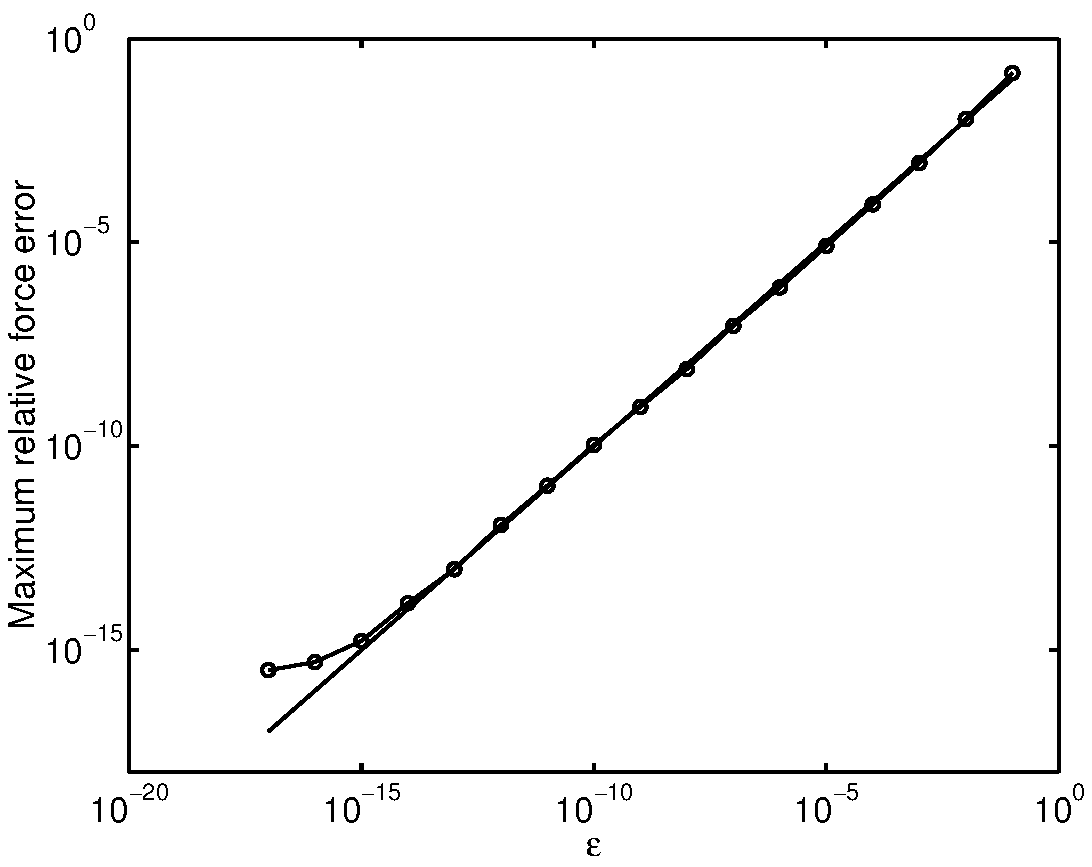
\includegraphics[width=6.5cm]{relativemaxerror.pdf}}
  \caption{The maximum force error for a given accuracy parameter $\epsilon$.\label{fig:relativemaxerror}}
%matlab
%y = [1.4229e-01 1.0638e-02 8.9157e-04 8.6253e-05 8.1670e-06 7.8197e-07 8.9641e-08 7.8154e-09 9.2093e-10 1.0716e-10 1.0669e-11 1.1634e-12 9.5996e-14 1.3959e-14 1.6625e-15 5.0350e-16 3.2148e-16];x=[1e-1 1e-2 1e-3 1e-4 1e-5 1e-6 1e-7 1e-8 1e-9 1e-10 1e-11 1e-12 1e-13 1e-14 1e-15 1e-16 1e-17];loglog(x,y,'-o',x,x,'-');axis ([1e-20 1 1e-18 1]);ylabel('Maximum relative force error');xlabel('\epsilon');scale(1.7);print -deps relativemaxerror.eps
\end{minipage}
\hfill
\begin{minipage}{6.6cm}
%matlab
%y = [1.48000 2.44000 3.50000 4.54000 7.10000 8.19000 9.45000 10.53000 11.64000 15.78000 17.16000 18.79000 20.40000 23.85000 25.60000 27.85000 29.81000 32.20000];x=[1e-1 1e-2 1e-3 1e-4 1e-5 1e-6 1e-7 1e-8 1e-9 1e-10 1e-11 1e-12 1e-13 1e-14 1e-15 1e-16 1e-17 1e-18];semilogx(x,y./(max(y)));axis ([1e-18 1e-1 0 1]);ylabel('Time');xlabel('\epsilon');scale(1.7);print -deps timmeaccuracy.eps
  \centerline{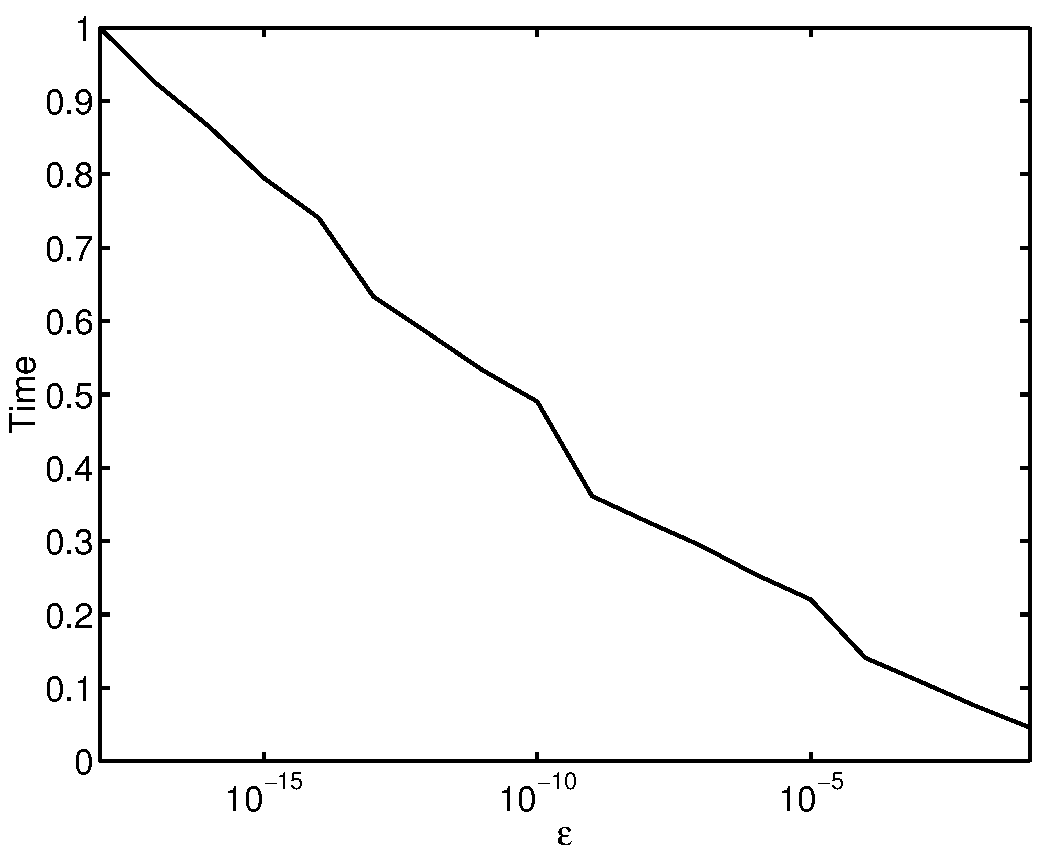
\includegraphics[width=6.5cm]{timmeaccuracy.pdf}}
  \caption{Normalized run-time  for a given accuracy
  parameter $\epsilon$.\label{fig:timmeaccuracy}}
\end{minipage}
\end{figure}


%%%%%%%%%%%%%%%%%%%%%%%%%%%%%%%%%%%%%%%%%%%%%%%%%%%%%%%%%%%%%%%%%%%%%%%%%
\subsubsection*{Choice of parameters}

The accuracy and performance of the Ewald summation is governed 
by the splitting factor $\alpha$, the real- and reciprocal-space term
cutoffs $r_c$ and $k_c$, and the accuracy $\epsilon$.
The splitting parameter $\alpha$ defines how
fast the sums converge and defines the cutoffs $r_c$ and $k_c$ for a given
accuracy $\epsilon$. For most applications, $r_c$ is small enough such that
$\vec{n} \in \{ \vec{0} \}$, which also simplifies the sum for the
real-space term. 
Both the real- and reciprocal-space term converge rapidly, such that
only a few terms need to be considered.
For the real part only terms satisfying $|\vec{x}_{ij} + \vec{n}| < r_c$ are
included, whereas for the reciprocal part only summands with $|\vec{k}|
< k_c$ are evaluated. 

From Eq.\ (\ref{eq:ewald}) it is obvious that for
a given accuracy and a fixed $\alpha$ the required work scales as
$\mathcal{O}(N^2)$ for the reciprocal term and as $\mathcal{O}(N)$ for
the real term. To achieve an overall work complexity of
$\mathcal{O}(N^{\frac{3}{2}})$, $\alpha$ must vary with $N$
\begin{eqnarray}
\alpha &=& c\sqrt{\pi} \left (  \frac{N}{V^2}\right )
^\frac{1}{6} 
\label{eq:ewald-alpha}\\
r_c  &=& \frac{\sqrt{-\ln \epsilon }}{\alpha}\label{eq:ewald-rc} \\
k_c &=& 2 \alpha \sqrt{-\ln \epsilon } ~.
\label{eq:ewald-kc}
\end{eqnarray}
Here, $V$ is the volume and the constant $c$ determines the ratio of
execution time of the real and reciprocal term, which may vary from one
platform to another. The standard Ewald summation is unsurpassed for
very high accuracy. It is relatively easy to implement and the desired
accuracy can be increased and controlled up to machine precision
without any additional programming effort (see Figure~\ref{fig:relativemaxerror}). Due to
these excellent properties, the Ewald method is often used as
reference for the evaluation of other methods with periodic
boundary conditions. A more detailed discussion for the optimal choice of
$\alpha$ and more accurate error estimates can be found in~\cite{DeHo98,Finc94,KoPe92,Pete95}.




%%%%%%%%%%%%%%%%%%%%%%%%%%%%%%%%%%%%%%%%%%%%%%%%%%%%%%%%%%%%%%%%%%%%%%%%%
\subsection{Mesh-based Ewald methods (PME)}

The mesh-based Ewald methods approximate the reciprocal-space term of
the standard Ewald summation by a discrete convolution on an
interpolating grid, using the discrete
Fast-Fourier transforms (FFT). By choosing an appropriate
splitting parameter $\alpha$, the computational cost
can be reduced from $\mathcal{O}(N^{\frac{3}{2}})$ to $\mathcal{O}(N \log
N)$. The accuracy and speed are additionally governed by the mesh size
and the interpolation scheme, which makes the choice of optimal
parameters more difficult. At present, there exist several
implementations based on this idea, but they differ in
detail. In \cite{DeHo98} three essential methods are compared and summarized:
particle-particle-particle-mesh~\cite{HoEa81} (P$^3$M), particle-mesh
Ewald~\cite{DaYP93} (PME) and smooth particle-mesh Ewald~\cite{EsPB95}
(SPME). 

Unfortunately, the mesh-based Ewald methods are
affected by errors when performing interpolation, FFT, and
\begin{figure}[bht]
\begin{minipage}{6.6cm}
  \centerline{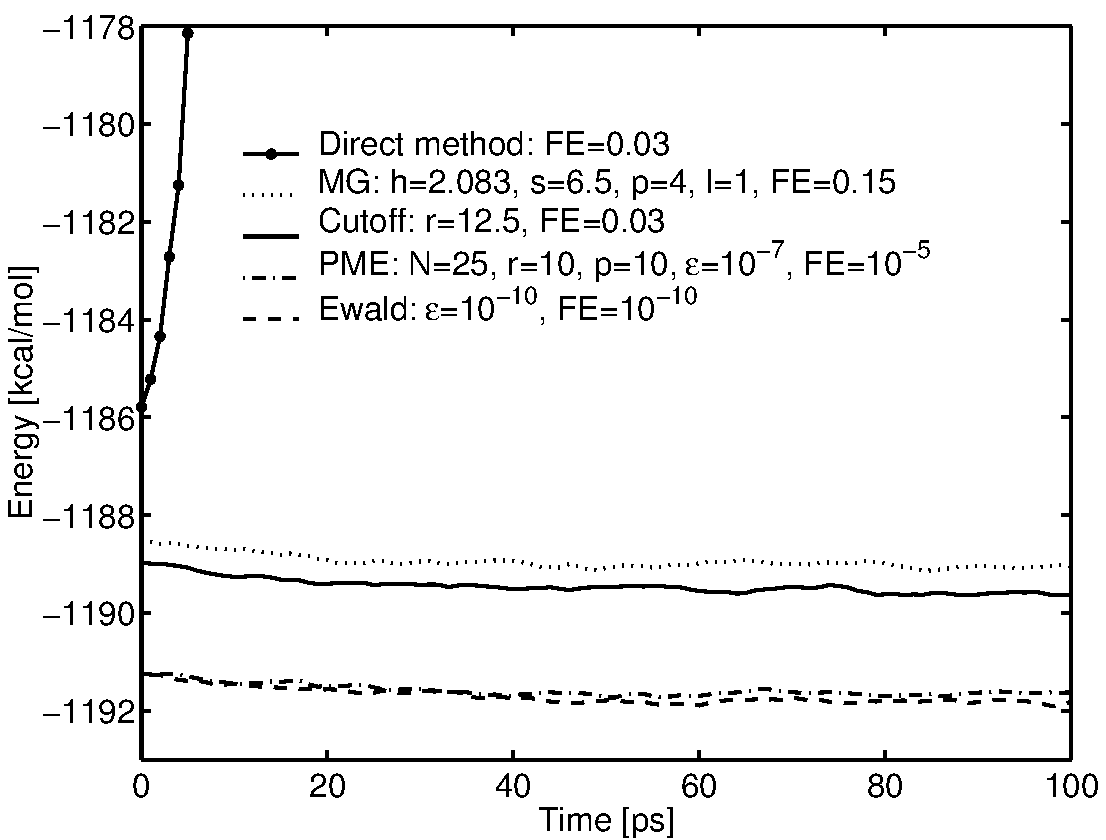
\includegraphics[width=6.5cm]{energydriftPBC.pdf}}
  \caption{The energy for periodic boundary conditions and step size 1 fs.\label{fig:energydriftPBC}}
\end{minipage}
\hfill
\begin{minipage}{6.6cm}
  \centerline{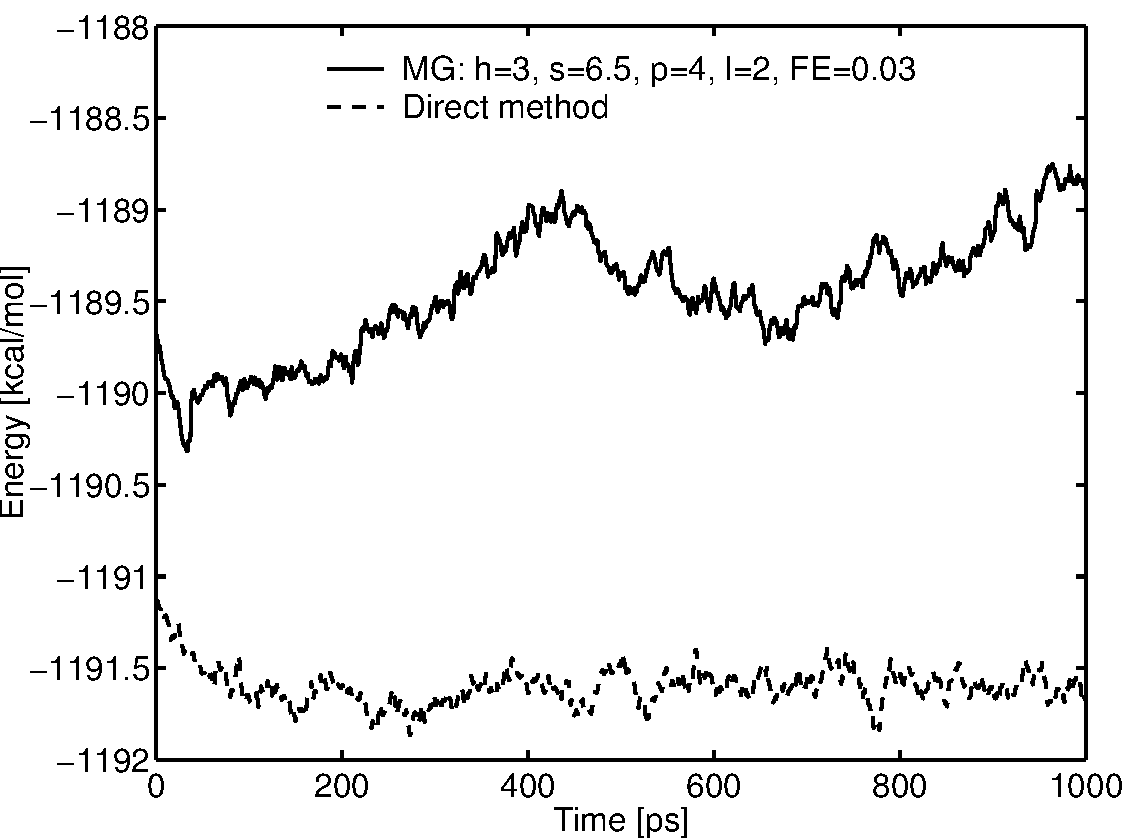
\includegraphics[width=6.5cm]{energydriftVacuum.pdf}}
  \caption{The energy for vacuum and step size 1 fs.\label{fig:energydriftVacuum}}
\end{minipage}
\end{figure}
differentiation~\cite{Pete95}. However, it would be misleading to
infer that these methods sacrifice accuracy in favor of run-time
performance.

For the fast mesh-based Ewald methods, there exists a critical number $N^*$ such that
they are faster than the standard Ewald method for $N>N^*$, due to the
fact of better scaling. In \cite{KaNa01}, the
computational efficiency and accuracy with 2-dimensional periodic
boundary conditions for 3-dimensional systems are discussed.\\

\ProtoMol\ supports PME with a generic
interpolation scheme interface
of arbitrary order. Actually, B-splines and Hermitian interpolation are
implemented. The  real, reciprocal and correction term can be evaluated
separately, as for the standard Ewald implementation. The real term
can be modified by a generic switching function. The implementation supports parallelism (range computation)
for the real and correction terms. The work of the reciprocal
term cannot be distributed in the actual implementation.

The maximum relative error of the PME method compared against the
standard Ewald summation is less than $2\cdot 10^{-14}$. Both methods
 used an accuracy parameter $\epsilon = 10^{-18}$. The PME was defined with mesh size of
0.1\AA , cutoff in real-space part $r_c = 10$, and B-splines  of order
12. Figure~\ref{fig:energydriftPBC} shows  excellent energy
conservation with a maximum relative force error of order $10^{-5}$.
NAMD2~\cite{Kale99} was used to validate the results.
%%%%%%%%%%%%%%%%%%%%%%%%%%%%%%%%%%%%%%%%%%%%%%%%%%%%%%%%%%%%%%%%%%%%%%%%
\subsection{Parameter Values}
\label{sec:ewald-auto}
%%%%%%%%%%%%%%%%%%%%%%%%%%%%%%%%%%%%%%%%%%%%%%%%%%%%%%%%%%%%%%%%%%%%%%%%

Both the real- and reciprocal-space series (the sums over $\bm{n}$ and
$\bm{k}$) converge fairly rapidly so that only a few terms need be
evaluated.  We define the \emph{cut-off} distances $r_c$ and $k_c$ so
that only terms with $| \bm{x}_{ij} +\bm{n} | < r_c$ and $|\bm{k}| < k_c$
are included.  The parameter $\alpha$ determines how rapidly the terms
decrease and the values of $r_c$ and $k_c$ needed to achieve a given
accuracy. 

For a fixed $\alpha$ and accuracy the number of terms in the
real-space sum is proportional to the total number of sites, $N$ but
the cost of the reciprocal-space sum increases as $N^2$. An overall
scaling of $N^\frac{3}{2}$ may be achieved if $\alpha$ varies with
$N$. This is discussed in detail in an excellent article by David
Fincham\cite{}.  The optimal value of $\alpha$ is
%
\begin{equation}
\alpha = \sqrt{\pi} \left ( \frac{t_R}{t_F} \frac{N}{V^2}\right )
^\frac{1}{6} 
\end{equation}
%
where $t_R$ and $t_F$ are the execution times needed to evaluate a
single term in the real- and reciprocal-space sums respectively.
If we require that the sums converge to an accuracy of $ \epsilon =
\exp ( -p )$ the cutoffs are then given by

\begin{eqnarray}
r_c  &=& \frac{\sqrt{p}}{\alpha} \\
k_c &=& 2 \alpha \sqrt{p}
\end{eqnarray}

A representative value of $t_R/t_F$ specific to \ProtoMol\ has been
established as 5.5.  Though this will vary on different processors
and for different potentials its value is not critical since it
enters the equations as a sixth root. \\
It must be emphasized that the $r_c$ is used as a cutoff for the
short-ranged potentials as well as for the electrostatic part.  The
value chosen above \emph{does not} take the nature of the
non-electrostatic part of the potential into account.  It is therefore
the responsibility of the user to ensure that $r_c$ is adequate for
this part too.\\

In case of Particle-Mesh Ewald sum, the reciprocal term is computed by
a Fourier transform. The cutoff $r_c$, $\alpha$ and $\epsilon$ are
chosen such as
\begin{equation}
  \frac {\erfc (\alpha r_c)}{r_c}= \epsilon 
\label{eq:pme-alpha}
\end{equation}.


%%%%%%%%%%%%%%%%%%%%%%%%%%%%%%%%%%%%%%%%%%%%%%%%%%%%%%%%%%%%%%%%%%%%%%%%%
\section{Input parameters}

This sections gives the definition of the plain Ewaldc for \ProtoMol. 

%%%%%%%%%%%%%%%%%%%%%%%%%%%%%%%%%%%%%%%%%%%%%%%%%%%%%%%%%%%%%%%%%%%%%%%%%
\subsection{General syntax plain Ewald}

\ProtoMol\  expects the following input plain Ewald:
\small
\begin{verbatim}
  Coulomb -algorithm FullEwald -real -reciprocal -correction
    -alpha     <real=-1>	
    -accuracy  <real=1e-05,positive>
    -j         <real=3,positive>     # Vacuum
 \end{verbatim}
\normalsize
, where \texttt{=}{\it value} defines the default value, i.e. optional
input.\\
Note that \texttt{Coulomb} can be replaced by a new, user defined potential,
which is of the form $c r^a$, where $c$ is a constant and $r$ is the
distance between particle pairs. For the Lennard-Jones potential a new
template is required due to the sum in the potential definition.
'\texttt{-j <real=3>}' is only available for vacuum.

%%%%%%%%%%%%%%%%%%%%%%%%%%%%%%%%%%%%%%%%%%%%%%%%%%%%%%%%%%%%%%%%%%%%%%%%%
\subsection{Real space term}

The flag \texttt{-real} emphasizes the computation of the real space term.

%%%%%%%%%%%%%%%%%%%%%%%%%%%%%%%%%%%%%%%%%%%%%%%%%%%%%%%%%%%%%%%%%%%%%%%%%
\subsection{Reciprocal space term}

The flag \texttt{-reciprocal} emphasizes the computation of the reciprocal space term.

%%%%%%%%%%%%%%%%%%%%%%%%%%%%%%%%%%%%%%%%%%%%%%%%%%%%%%%%%%%%%%%%%%%%%%%%%
\subsection{Correction  space term}

The flag \texttt{-correction} emphasizes the computation of the
resting terms in Eq. \ref{eq:ewald}: 
point self term, intra-molecular self term, charged system term
and surface dipole term. Note that the surface dipole term is not considered in the actual implementation.

%%%%%%%%%%%%%%%%%%%%%%%%%%%%%%%%%%%%%%%%%%%%%%%%%%%%%%%%%%%%%%%%%%%%%%%%%
\subsection{Switching function}
The switching function is by default an ordinary cutoff. If an other
switching function is required, one must register the corresponding
prototype in the according factory.

%%%%%%%%%%%%%%%%%%%%%%%%%%%%%%%%%%%%%%%%%%%%%%%%%%%%%%%%%%%%%%%%%%%%%%%%%
\subsection{Accuracy}

The optional parameter \texttt{-accuracy <real>} defines the accuracy
of the splitting. By default \ProtoMol\ will use an accuracy of
$1e-06$.

%%%%%%%%%%%%%%%%%%%%%%%%%%%%%%%%%%%%%%%%%%%%%%%%%%%%%%%%%%%%%%%%%%%%%%%%%
\subsection{Splitting of the sum -- alpha}


The optional parameter $\alpha$ (\texttt{-alpha <real>}) determines how rapidly
the terms
decrease and the values of cutoff (real space term) $r_c$ and lattice
cutoff (reciprocal space term) $k_c$ needed to achieve a given
accuracy. $\alpha$ is the so-called splitting parameter of the Ewald
summation. $\alpha \in (0,1)$, where $0^+$ and$1^-$ means only real
space or reciprocal space term, respectively. By default \ProtoMol\ will compute depending on the cutoff and for
the given accuracy, Eq. \ref{eq:ewald-kc},\ref{eq:pme-alpha}.

%%%%%%%%%%%%%%%%%%%%%%%%%%%%%%%%%%%%%%%%%%%%%%%%%%%%%%%%%%%%%%%%%%%%%%%%%
\subsection{J -- expansion factor for vacuum}

In order to make PME work with vacuum we add a
shell around the actual simulation box (bounding box of all particles)
to be able to use PME together with periodic boundary conditions. With a large enough shell we can mimic vacuum. By default \ProtoMol\ will use a factor of 3, which
means it will add 1 simulation boxes in each dimension (see
Fig. \ref{fig:expansion}), or in other words expanding the simulation
box by a factor 3.
\begin{figure}[hbt]
  \centerline{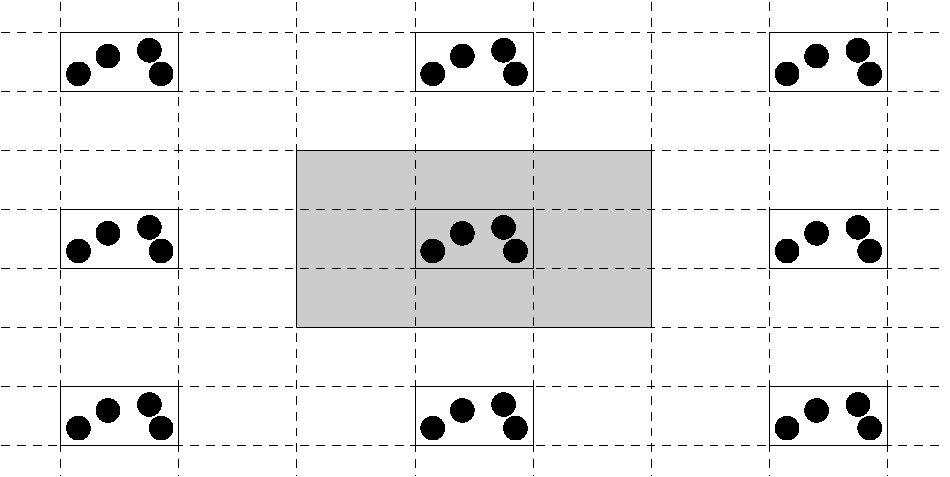
\includegraphics[width=5cm]{expansion.pdf}}
  \caption{Example of expansion factor of 3 in 2d.}
  \label{fig:expansion}
\end{figure}


%%%%%%%%%%%%%%%%%%%%%%%%%%%%%%%%%%%%%%%%%%%%%%%%%%%%%%%%%%%%%%%%%%%%%%%%%
\subsection{Compilation}

For experimental purpose the Ewald has several conditional compilation
flags.\\
\begin{tabular}{cp{10cm}}
\texttt{\small DEBUG\_PME\_TIMING}        & Printing the different timings\\
\texttt{\small DEBUG\_PME\_ENERGIES}      & Printing the different energy contributions\\
\texttt{\small USE\_PME\_EXACT\_SOLUTION}& Using the exact solution of erf() in the real part\\
\end{tabular}

%%%%%%%%%%%%%%%%%%%%%%%%%%%%%%%%%%%%%%%%%%%%%%%%%%%%%%%%%%%%%%%%%%%%%%%%%
\subsection{General syntax PME}

\ProtoMol\  expects the following input for PME:
\begin{verbatim}
  Coulomb -algorithm PMEwald -correction -interpolation BSpline
    -gridsize   <uint,positive> <uint,positive> <uint,positive>
    -cutoff     <real,positive>
    -order      <uint=4,positive>	
    -accuracy   <real=1e-06,positive>
    -alpha      <real=-1>
    -j          <real=3>
\end{verbatim}
, where \texttt{=}{\it value} defines the default value, i.e. optional
input.\\
Note that \texttt{Coulomb} can be replaced by a new, user defined potential,
which is of the form $c r^a$, where $c$ is a constant and $r$ is the
distance between particle pairs. For the Lennard-Jones potential a new
template is required due to the sum in the potential definition.
'\texttt{-j <real=3>}' is only available for vacuum.

%%%%%%%%%%%%%%%%%%%%%%%%%%%%%%%%%%%%%%%%%%%%%%%%%%%%%%%%%%%%%%%%%%%%%%%%%
\subsection{Real space term}

The flag \texttt{-real} emphasizes the computation of the real space term.

%%%%%%%%%%%%%%%%%%%%%%%%%%%%%%%%%%%%%%%%%%%%%%%%%%%%%%%%%%%%%%%%%%%%%%%%%
\subsection{Reciprocal space term}

The flag \texttt{-reciprocal} emphasizes the computation of the reciprocal space term.

%%%%%%%%%%%%%%%%%%%%%%%%%%%%%%%%%%%%%%%%%%%%%%%%%%%%%%%%%%%%%%%%%%%%%%%%%
\subsection{Correction  space term}

The flag \texttt{-correction} emphasizes the computation of the
resting terms in Eq. \ref{eq:ewald}: 
point self term, intra-molecular self term, charged system term
and surface dipole term. Note that the surface dipole term is not considered in the actual implementation.

%%%%%%%%%%%%%%%%%%%%%%%%%%%%%%%%%%%%%%%%%%%%%%%%%%%%%%%%%%%%%%%%%%%%%%%%%
\subsection{Interpolation}

\texttt{-interpolation} defines the interpolation scheme between the
grids the particle level. For the moment \ProtoMol\
does only accept b-splines interpolation (\texttt{BSpline}). Other
interpolations like Hermitian (\texttt{Hermite}) did not improve the
accuracy.

%%%%%%%%%%%%%%%%%%%%%%%%%%%%%%%%%%%%%%%%%%%%%%%%%%%%%%%%%%%%%%%%%%%%%%%%%
\subsection{Switching function}
The switching function is by default an ordinary cutoff. If an other
switching function is required, one must register the corresponding
prototype in the according factory.

%%%%%%%%%%%%%%%%%%%%%%%%%%%%%%%%%%%%%%%%%%%%%%%%%%%%%%%%%%%%%%%%%%%%%%%%%
\subsection{Gridsize}
\texttt{-gridsize <uint,positive> <uint,positive> <uint,positive>} defines the grid for the
reciprocal space term using FFT. The grid size should be shosen such that
\begin{equation}
  n_i = c e_i  \left ( \frac{N}{V} \right )
^\frac{1}{3} 
\end{equation}
is satisfied for some $c$. 

%%%%%%%%%%%%%%%%%%%%%%%%%%%%%%%%%%%%%%%%%%%%%%%%%%%%%%%%%%%%%%%%%%%%%%%%%
\subsection{Cutoff}
\texttt{-cutoff <real>} defines the cutoff of the real space term.

%%%%%%%%%%%%%%%%%%%%%%%%%%%%%%%%%%%%%%%%%%%%%%%%%%%%%%%%%%%%%%%%%%%%%%%%%
\subsection{Order}

The optional parameter \texttt{-order} defines the interpolation order. The interpolation
order must be even, where 4 and 6 stand for a {\it cubic} and 
{\it quintic} interpolation respectively. By default \ProtoMol\ will use 4th order interpolation.

%%%%%%%%%%%%%%%%%%%%%%%%%%%%%%%%%%%%%%%%%%%%%%%%%%%%%%%%%%%%%%%%%%%%%%%%%
\subsection{Accuracy}

The optional parameter \texttt{-accuracy <real>} defines the accuracy
of the splitting. By default \ProtoMol\ will use an accuracy of
$1e-06$.

%%%%%%%%%%%%%%%%%%%%%%%%%%%%%%%%%%%%%%%%%%%%%%%%%%%%%%%%%%%%%%%%%%%%%%%%%
\subsection{Splitting of the sum -- alpha}


The optional parameter $\alpha$ (\texttt{-alpha <real>}) determines how rapidly
the terms
decrease and the values of cutoff (real space term) $r_c$ and lattice
cutoff (reciprocal space term) $k_c$ needed to achieve a given
accuracy. $\alpha$ is the so-called splitting parameter of the Ewald
summation. $\alpha \in (0,1)$, where $0^+$ and$1^-$ means only real
space or reciprocal space term, respectively. By default \ProtoMol\ will compute depending on the cutoff and for
the given accuracy, Eq. \ref{eq:ewald-kc}\ref{eq:pme-alpha}.

%%%%%%%%%%%%%%%%%%%%%%%%%%%%%%%%%%%%%%%%%%%%%%%%%%%%%%%%%%%%%%%%%%%%%%%%%
\subsection{J -- expansion factor for vacuum}

In order to make PME work with vacuum we add a
shell around the actual simulation box (bounding box of all particles)
to be able to use PME together with periodic boundary conditions. With a large enough shell we can mimic vacuum. By default \ProtoMol\ will use a factor of 3, which
means it will add 1 simulation boxes in each dimension (see
Fig. \ref{fig:expansion}), or in other words expanding the simulation
box by a factor 3.


%%%%%%%%%%%%%%%%%%%%%%%%%%%%%%%%%%%%%%%%%%%%%%%%%%%%%%%%%%%%%%%%%%%%%%%%%
\subsection{Compilation}

For experimental purpose the Ewald has several conditional compilation
flags.\\
\begin{tabular}{cp{10cm}}
\texttt{\small DEBUG\_PME\_TIMING}        & Printing the different timings\\
\texttt{\small DEBUG\_PME\_ENERGIES}      & Printing the different energy contributions\\
\texttt{\small USE\_PME\_EXACT\_SOLUTION}& Using the exact solution of erf() in the real part\\
\end{tabular}


\bibliographystyle{abbrv}
\bibliography{lcls}
%%%%%%%%%%%%%%%%%%%%%%%%%%%%%%%%%%%%%%%%%%%%%%%%%%%%%%%%%%%%%%%%%%%%%%%%%
\end{document}
%%%%%%%%%%%%%%%%%%%%%%%%%%%%%%%%%%%%%%%%%%%%%%%%%%%%%%%%%%%%%%%%%%%%%%%%%
